\documentclass[a4paper]{article}

\usepackage[margin=1in]{geometry}
\usepackage{amsfonts, amsmath, mathrsfs}
\usepackage{graphicx}
\usepackage{hyperref}

\newcommand{\C}{\mathbb{C}}
\newcommand{\R}{\mathbb{R}}
\newcommand{\Q}{\mathbb{Q}}
\newcommand{\Z}{\mathbb{Z}}

\begin{document}

\begin{center}
\LARGE{Allen Hatcher - Algebraic Topology}

\Large{Chapter 2: Homology}

\large{Carter Hinsley's notes}

Rendered \today
\end{center}

\section{Singular homology}

Singular homology seems as though it should look like the image of simplicial homology under arbitrary continuous maps into other spaces.

A \emph{singular $n$-simplex} in a space $X$ is a (continuous) map $\sigma : \Delta^n \to X$. That is, it is \textbf{precisely} the map and not its image nor its domain. Let $C_n(X)$ be the free abelian group with basis the set of singular $n$-simplices in $X$. $C_n(X)$ is the group of \emph{(singular) $n$-chains} in $X$. The boundary map $\partial_n : C_n(X) \to C_{n-1}(X)$ is defined in the same way as in simplicial homology:
\begin{align}
    \partial_n(\sigma) = \sum_i (-1)^i \sigma | [v_0, \ldots, \hat{v}_i, \ldots, v_n].
\end{align}
Since this is a group homomorphism, it extends up from the basis formed by $\sigma$s to the whole group $C_n(X)$. Recall that $\sigma|[v_0, \ldots, \hat{v}_i, \ldots, v_n]$ is the restriction of $\sigma$ to the $n-1$-simplex missing $v_i$. You can really think of this as being a map $\sigma|[v_0, \ldots, \hat{v}_i, \ldots, v_n] : \Delta^{n-1} \to X$.

Here's an example in the case of simplicial homology:
\begin{center}
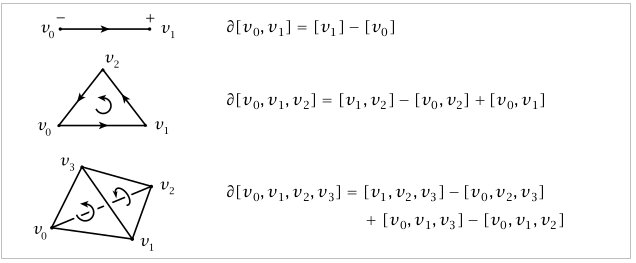
\includegraphics[width=5in]{graphics/simplicial_boundaries.png}
\end{center}

Letting $\partial_0 : C_0(X) \to 0$, the boundary maps $\partial_n$ form a long exact chain called a \emph{chain complex}. Thus we define the $n$th singular homology group $H_n(X) = \ker \partial_n / \text{im } \partial_{n+1}$.

Any two homeomorphic spaces will clearly have isomorphic singular homology groups.

It turns out that, counterintuitively, singular homology is a special case of simplicial homology. For an arbitrary space $X$, define the \emph{singular complex} $S(X)$ to be the $\Delta$-complex with one $n$-simplex $\Delta_\sigma^n$ for each singular $n$-simplex $\sigma : \Delta^n \to X$, with $\Delta_\sigma^n$ attached in the obvious way to the $(n-1)$-simplices of $S(X)$ that are the restrictions of $\sigma$ to the various $(n-1)$-simplices in $\partial \Delta^n$. Now observe that $H_n^\Delta(S(X))$ is identical to $H_n(X)$ for all $n$. One can regard $S(X)$ as a $\Delta$-complex model for $X$, but it's usually extremely large compared to $X$.

\end{document}